\documentclass[letterpaper]{article}
\usepackage{aaai16}
\usepackage[table]{xcolor}
\usepackage{graphicx}
\usepackage{amssymb}
\usepackage{hyperref}
\usepackage[vlined,ruled,linesnumbered]{algorithm2e}
\usepackage{algpseudocode}
\usepackage{float}
\usepackage{tikz}
\usepackage{color}
\usepackage{calc}
\usepackage{times}
\usepackage{helvet}
\usepackage{courier}
\usetikzlibrary{automata, positioning}
\frenchspacing
\setlength{\pdfpagewidth}{8.5in}
\setlength{\pdfpageheight}{11in}
\pdfinfo{
/Title (Insert Your Title Here)
/Author (a,b,c,d)}
\setcounter{secnumdepth}{0}
 \begin{document}
% The file aaai.sty is the style file for AAAI Press
% proceedings, working notes, and technical reports.
%
\title{Formatting Instructions test \\for Authors Using test \LaTeX{}}
\author{AAAI Press_1\\
Association for the Advancement of Artificial Intelligence\\
1.2275 East Bayshore Road, Suite 160\\
Palo Alto, California 94303\\
}
\maketitle


\newcommand{\X}{\mathcal{X}}
\newcommand{\g}{\mathcal{G}}
\newcommand{\var}{\textsf{var}}
\newcommand{\Lit}{{\cal L}}

\newcommand {\SAT}{\textsf{SAT}}
\newcommand {\MUC}{\textsf{MUC}}
\newcommand{\degr}{\textsf{d}}
\newcommand{\BL}{\textsf{BL}}
\newcommand{\BLap}{{\sf \widehat{BL}}}
\newcommand{\NBLap}{{\sf \overline{BL}_\downharpoonright}}
\newcommand{\BV}{\textsf{BV}}
\newcommand{\HDBS}{\textsf{HDBS}\xspace}

\newcommand{\tool}{{\sc Bone}\xspace}
\newcommand{\NBV}{\overline{\textsf{BV}}}
\newcommand{\NBL}{\overline{\textsf{BL}}}
\newcommand{\NBC}{\overline{\textsf{BC}}}

\newcommand{\HBL}{{\sf HBL}\xspace}

\newcommand{\cls}{\textsf{cls}}
\newcommand{\cl}{\mathcal{C}}
\newcommand{\f}{\textsf{F}}
\newcommand{\Cnt}{\textsf{Cnt}}
\newcommand{\dens}{\textsf{Dnt}}
\newcommand{\NB}{{\bf NB$\downharpoonright$}}
\newcommand{\MBNB}{{\bf MBNB$\downharpoonright$}}
\newcommand{\HBNB}{{\bf HBNB$\downharpoonright$}}
\newtheorem{theorem}{Theorem}
\newtheorem{lemma}{Lemma}
\newtheorem{corollary}{Corollary}
\newtheorem{proposition}{Proposition}
\newtheorem{definition}{Definition}
\newtheorem{example}{Example}
\newtheorem{remark}{Remark}


% \title{Computing backbone variables using approximations}

%\author{Yueling Zhang
%\and Min Zhang
%\and Fu Song
%\and Geguang Pu
}

% (feature abused for this document to repeat the title also on left hand pages)

% the affiliations are given next; don't give your e-mail address
% unless you accept that it will be published
%\institute{Computer Science and Software Engineering Institute, East China Normal University,\\
%North Zhongshan Rd. 3663, 200062 Shanghai, China\\
%yueling671231@163.com\\
%\{ mzhang, fsong, ggpu\}@sei.ecnu.edu.cn\\}

\begin{abstract}
Backbone Variables are widely used in random SAT solving, all-sat computing and SAT based model checking. In this paper, we propose several novel approaches to finding backbone variables using modern SAT solvers and approximations.
Experiments show the efficiency of the approaches using satisfiable instances from SAT Comp.2015. Moreover, compared with state-of-the-art approach proposed in 2014, our approaches has obvious advantages.
\end{abstract}

\section{Introduction}

Backbones are firstly generalized from the coloring problem. A pair of nodes are backbones if they always have the same color in every possible k-coloring\cite{WTS2001}.

In satisfiability problem, given a formulae $\Phi$, an truth assignment is a map from boolean variables to literals appeared in $\Phi$. In an assignment, a literal can only be assigned as TRUE or FALSE. Given an assignment $\lambda$, if there exist at least one literal in a clause $\phi\in\Phi$ that has been assigned as TRUE according to $\lambda$, $\phi$ is called to be satisfied by $\lambda$. If there exists a $\lambda$ that satisfy every clause $\phi\in\Phi$, $\lambda$ is a model or a satisfied assignment of $\Phi$.
Backbones of a propositional formula $\Phi$ is a cluster of literals that are TRUE in every model of $\Phi$\cite{BCJ2001,KPJ2005}.

Backbones have been studied in random 3-SAT problems \cite{DOG2001}, optimization problems\cite{CJG2001,KPS2005,WTS2001}, as well as Maximal Satisfiability(MSS) problems\cite{MM2005}.
As shown in \cite{ZWR2003}, backbones are applied to local minima of Walksat and improves the performance of Walksat by making biased moves in a local search. Another similar application of backbones information is shown in \cite{ZWL2005}, in this experiment, backbones information significantly contributes to the acceleration of Lin-Kernighan(LK) local search family algorithms when dealing with Travel Salesman Problem(TSP).
A more recent application of backbones arises in \cite{Z11}. A number of backbones extracting approaches are proposed and applied to post silicon fault localisation. The results show that backbones extracting using SAT solvers are suitable for large scale applications with only a little SAT solver calls.

As shown above, finding backbones is the key in many practical applications, such as planning problem and constraint satisfaction problem. It has been proved that backbones computing is a co-NP problem\cite{Jan10}, which have rise huge challenges.
A number of backbones extraction algorithms have been proposed in recent years. All state-of-the-art backbones extraction approaches employ SAT solvers, MiniSAT\cite{MINISAT} for most of them.
Implicant enumeration\cite{MK2002,RSF2004} enumerates implicants of formula $\Phi$ one by one and updates the backbones estimation in each iteration. The negation of an implicant is added to $\Phi$ in order to avoid finding the same implicant. For an implicant $\lambda$, the negation of $\lambda$ is $\bigvee_{l\in\lambda}\neg l$. Standard implicants reducing techniques can be applied to mitigate the size of blocking clauses. It have to enumerate all models of $\Phi$ before the algorithm terminates, which is unnecessary costly.

Zhu et al, proposed an iterative SAT testing algorithm \cite{Z11}. The algorithm maintains an estimation of backbones $\Phi_\BL$. The negation of $\Phi_\BL$ is the disjunction of each complementing literals in backbones estimation, i.e., $\neg\Phi_\BL=\bigvee_{\neg l}, l\in\Phi_\BL$. In each iteration, a clause that formed by $\neg \Phi_\BL$ conjuncted to $\Phi$ and formed $\Phi'$. If $\Phi'$ is satisfiable, it means that at least one non-backbone is in the backbone estimation, estimation is refined by removing the non-backbone literal. The process is repeated until $\Phi'$ is not satisfiable any longer. Along with the estimation, the clauses number of $\Phi'$  is monotone increasing due to the continuously disjunction in each iteration, which dramatically promote the complexity of $\Phi'$. In other words, for each iteration, it takes longer CPU time than the last iteration.

The Core Based Algorithm presented in \cite{JLM15} is stable and effectiveness. It considers complementing of the model as assumptions input for SAT solver in each iteration. If $\Phi$ is unsatisfied under given assumptions, a core is returned by SAT solver to indicate reasons. According to the implementation of MiniSAT 2.2 \cite{MINISAT}, the reason is a part of the given assumptions. Whenever there is exactly one literal in the reason, the literal is a backbone. If there is more than one literal in the reason, they will be marked as visited. If every literal in an iteration is visited, iterative SAT testing will be invoked to test the rest of unmarked literals. According to the author, for the lower percentages of backbones, Core Based Algorithms are significantly better. When the percentage of backbone is over 25\%, Core Based Algorithm behave very similarly Iterative SAT Testing Algorithm.

Revisited previous researches, backbones computing of low density backbones formulae is quiet efficiencies and efficiency. In this paper, we focus on the hard instance, proposed a novel approach to spot non-backbones ahead and to estimate backbones. Instead of accumulating clauses to formula like Iterative SAT testing does, we test the literals one by one by leveraging assumptions. Assumptions are a group of literals. We consider assumptions as a kind of constraint input, it means that the literals in assumptions must be assigned to true in an assignment. If there exists a model $\lambda$ such that it satisfy every literals in assumptions, the formula is satisfied under these assumptions. According to the satisfiability theory, assumptions are equivalence to clauses that only contains the assumption literal. Compared with clauses conjunction, assumptions won't increase the complexity of formula since no clauses are added to the formula. Also, assumptions is more suitable for iterative SAT testing since it can be reset in each iteration.

Using variables clauses coverage analysis, a group of non-backbone literals and an estimation of backbones are obtained, refereed as $\NBL_u$ and $\HDBS$, respectively. For each literals in $\HDBS$, Minisat with assumptions will be evoked. The only assumption in each iteration is the current testing literal. If Minisat returns false, the literal is a backbone, it will be conjuncted with the original formula to simplify it.

The approach leveraging Whitening Algorithm and other pervious backbones computing algorithms, designed and implemented a Multi Estimation Based Algorithms (MEB) , experiments are conducted to evaluate MEB, results showed that MEB is compatible with Core Based Algorithm when dealing with low density backbones formulae. For hard formulae with dense backbones, MEB outperforms Core Based Approach considering the total SAT solver time and SAT calls number.
Compared with Core Based Algorithm which directly calculate backbones. MEB estimate non-backbone literals and backbone literals ahead.
Unlike the Iterative SAT Testing approach, the estimation doesn't need to rely on SAT solvers. Only one SAT solver call is needed during the estimation process. 
%FCB will first compute the under-approximation of non-backbone literals, referred as $\NBL_u$ in $O(n^2)$ time. With the $\NBL_u$ information, a group of literals with dense backbones will be estimated in polynomial time, refereed as $\HDBS$.
%Iterative SAT testing per literals of $\HDBS$ will be applied to determine whether a literal is a backbone or not. A backbone literal will be conjuncted with formula as a new unit clause. With several backbones, formula will be simplified\cite{MPA2015}.
Experiments indicate that, the average dense of backbones in $\HDBS$ is over 50\%, which helps MEB to recognize more backbones in less SAT solver calls than CB needs. Especially for hard formulae, MEB will save a large amount of CPU time since it invoking less Minisat than CB does.

This paper is organized as follows.
Section 2 introduces the concept of backbones.
Section 3 relates backbones estimate reducing procedures to Core Based Backbones Extraction Algorithms and evolved to Filter Core Based(FCB) Backbone Extraction Algorithms.
Section 4 presents the experimental evaluation of FCB.
Section 5 makes a conclusion and discusses about future work.

\section{Preliminaries}\label{sec:prel}

We fix a finite set  $\X$ of \emph{Boolean variables}.
A \emph{literal} $l$ is either a Boolean variable $x\in \X$ or its negation $\neg x$.
The negation of a literal $\neg x$ is $x$, i.e., $\neg\neg x=x$.
A \emph{clause} $\phi$ is a disjunction of literals $\bigvee_{i=1}^n l_i$, which may be regarded as
the set of literals $\{l_i\mid 1\leq i\leq n\}$.

A \emph{formula} $\Phi$ over $\X$ is a Boolean combination of variables $\X$.
We assume that formulae are given in conjunctive normal
form (CNF), namely each formula $\Phi$ is a conjunction of clauses $\bigwedge_{i=1}^n\phi_i$ which may be regarded as a set of clauses $\{\phi_i\mid 1\leq i\leq n\}$.
Given a formula $\Phi$, let $\var(\Phi)$ (resp. $\Lit(\Phi)$  and $\cls(\Phi)$) denote the set of variables (resp. literals and clauses) used in $\Phi$.
We use $\neg\Lit(\Phi)$ to denote the set $\{\neg l \mid l\in \Lit(\Phi)\}$.
The \emph{size} $|\Phi|$ of $\Phi$ is the number of literals of $\Phi$.
Given a formula $\Phi$ and a literal $l\in\Lit(\Phi)$,
let $\Phi_{l}\subseteq \Phi$ be the set of clauses $\{\phi\in\Phi\mid l\in\phi\}$.
%and $\Phi_\downarrow$ be the set $\{(l,\Phi_{\downarrow l})\mid l\in \Lit(\Phi)\}$.
%Given a clause $\phi$ of $\Phi$, let $\sharp(\phi,\Phi)$ be the count of occurrence of $\phi$ in the second components of tuples in $\Phi_\downarrow$.
%Given a set of clauses $\Phi_{l_x}$, let $\Phi_{l_x}^0 = \Phi_{\downarrow l}$, let $\Phi_{\downarrow l}^k$, $\Phi_{\downarrow l}^{k-1}\subseteq\Phi_{\downarrow l}^k\subseteq\Phi_{\downarrow 1}^{k+1}\subseteq\Phi (k \geq 1)$ be the set of clauses $\{\phi\in\Phi \mid \exists l\in\Lit(\Phi_{\downarrow l}^{k-1}), \neg l\in\Lit(\phi)\} (k \geq 1)$.

%A \emph{partial assignment} is a partial function $\lambda:\X\rightarrow \{0,1\}$ which assigns to each defined variable a Boolean value. Let $\lambda_x$ denote the partial assignment such that for every $y\in \X$, $\lambda_x(y)=\lambda(x)$ if $x=y$, otherwise $\lambda_x(y)$ is undefined.
%A \emph{complete assignment} is a partial assignment in which all the variables are defined.

An \emph{assignment} is a function $\lambda: \X \rightarrow \{0,1\}$, where $1$ (resp. $0$) denotes true (resp. false).
Given an assignment $\lambda$ and a literal $l$ that is $x$ or $\neq x$, let $\lambda[\neg l]$ be the assignment which is equal to $\lambda$
except for $\lambda[\neg l](x)=\neg \lambda(x)$.
An assignment $\lambda$ \emph{satisfies} a formula $\Phi$, denoted by $\lambda\models \Phi$, iff assigning $\lambda(x)$ to $x$ for $x\in\var(\Phi)$ makes $\Phi$ true.
An assignment $\lambda$ is a \emph{model} of $\Phi$ if $\lambda\models \Phi$.
A formula $\Phi$ is \emph{satisfiable} iff there exists an assignment $\lambda$ such that $\lambda\models \Phi$.
%A variable $x\in\phi$ \emph{satisfies} a formula $\Phi$, denoted by $x\models\Phi$, iff assigning $1$ to $x$ makes with its value $\lambda(x)$.
Given a formula $\Phi$, the \emph{satisfiability problem} is to decide whether $\Phi$ is satisfiable or not.
%Whenever convenient, a formula $\Phi$ is seen as a set $\cls(\Phi)$ of clauses, a clause $\phi$ is seen as a set $\Lit(\phi)$ of literals, and an assignment %$\phi$ is seen as a set of clauses.
%In the rest of this section, we will introduce several technical concepts, amendable to our approach.

\smallskip
%Given an unsatisfiable Boolean formula $\Phi$, an \emph{unsatisfiable core} is a subset of clauses $C\subseteq \cls(\Phi)$ such that
%$\Phi_C$ is still unsatisfiable. An unsatisfiable core $C$ of $\Phi$ is called a \emph{minimal unsatisfiable core} if
%for every $C'\subset C$, $\Phi_{C'}$ is satisfiable. Intuitively, unsatisfiable core is a minimal unsatisfiable core it is unsatisfiable, but removing any of %its clauses makes it satisfiable.

\begin{definition}[Backbone]
\label{def:backbone}
Given a satisfiable formula $\Phi$, a literal $l$ is a \emph{backbone literal} of $\Phi$ iff for all assignments $\lambda$ such that $\lambda\models\Phi$,
$\lambda\models l$. The \emph{backbone} $\BL(\Phi)$ of $\Phi$ is the set of backbone literals of $\Phi$.
\end{definition}



%\begin{definition}[Nonbackbone]
%\label{def:backbone}
%Given a satisfiable formula $\Phi$, a variable $x\in\var(\Phi)$ is a \emph{nonbackbone variable} of $\Phi$ iff there exist two satisfying assignments
%$\lambda_1$ and $\lambda_2$ such that $\lambda_1(x)\neq \lambda_2(x)$.
%A clause $\phi\in \Phi$ is \emph{nonbackbone clause} iff $|\var(\phi)|\geq 2$ and there is a nonbackbone variable of $\Phi$ in $\phi$.
%For an unsatisfiable formula $\Phi$, the set of nonbackbone variables is $\var(\Phi)$.
%\end{definition}
It is known that the backbone $\BL(\Phi)$ for each formula $\Phi$ is unique and a backbone literal $l$ of $\Phi$ must be in
$\BL(\Phi)$ \cite{JLM15}.
The backbone of an unsatisfiable formula can be defined as an empty set. Therefore, in this work, we focus on satisfiable formulae.
We will use $\NBL(\Phi)$ to denote the set
$\Lit(\Phi)\setminus \BL(\Phi)$.

\begin{theorem}
\label{thm:co-NP}\cite{Jan10}
Given a satisfiable formula $\Phi$ and a literal $l$, deciding whether $l$ is a backbone literal is co-NP-complete.
\end{theorem}

% \begin{definition}[Model]
% Given a satisfied formula $\Phi$, a model $\lambda$ is a truth assignment such that $\lambda\models\Phi$.
% \end{definition}

\begin{definition}[Satisfied literal]
Given a model $\lambda$ of the formula $\Phi$ and a clause $\phi\in\Phi$, for each literal $l\in\phi$, $l$ is a \emph{satisfied literal}
of $\phi$ iff $\lambda\models l$. $l$ is a \emph{unique satisfied literal} of $\phi$ if there is no satisfied literal $l'$ of $\phi\setminus\{l\}$.
\end{definition}

%\begin{definition}[Unique satisfied literal]
%Given a satisfied formula $\Phi$, a model $\lambda$, a clause $\phi\in\Phi$, a satisfied literal $l$, $l$ is a unique satisfied literal iff %there
%exist exactly only one satisfied literal $l$ in $\phi$ with the assignment of $\lambda$.
%\end{definition}

%\begin{example}
Let us consider the formula $\Phi=\{\neg x_1 \vee \neg x_2, x_1, x_3 \vee x_4\}$,
$\var(\Phi)=\{x_1, x_2, x_3, x_4\}$, $\Lit(\Phi)=\{\neg x_1, x_1, \neg x_2, x_3, x_4\}$, $\Phi_{\neg x_2}=\{\neg x_1 \vee \neg x_2\}$ and $\BL(\Phi)=\{x_1, \neg x_2\}$.
%\end{example}


\begin{definition}[Literals Frequency]
Given a formula $\Phi$, the \emph{Frequency} of a literal $l\in\Lit(\Phi)$ is the number of clauses that contain $l$, refereed as $\f(l)$.
\end{definition}

\begin{definition}[Literals Density]
Given a formula $\Phi$, the \emph{Density} of a literal $l\in\Lit(\Phi)$ is the ratio of the frequency of the literal to the total length of clauses that contain the literal, refereed as $\d(l)$, i.e., $\d(l)=\f(l)\div|\Phi_l|$.
\end{definition}
%\begin{remark}\label{rem:na}
%Given a formula $\Phi$,
%a na\"{\i}ve approach for computing $\BL(\Phi)$ is to verify whether a set $B$ is a backbone or not by calling SAT solver, for every $B\subseteq \var(\Phi)$. %However, this naive approach has to call $2^{|\var(\Phi)|}$ times SAT solver in the worst case \cite{JLM15}.
%\end{remark}

\section{Overview of our Approach}\label{sec:walg}
\begin{figure*}
\centering
    \includegraphics[scale=0.9]{Framework}
   \caption{Overview of our approach}
   \label{flow}
\end{figure*}

Figure \ref{flow} presents the overview of our approach \tool, which consists of three components. Taking a satisfiable formula
$\Phi$ as an input, \tool first computes an under-approximation $\NBLap(\Phi)\subseteq \NBL(\Phi)$ of the non-backbone of
$\Phi$. Then, \tool computes an approximation $\BLap(\Phi)$ of the backbone of $\Phi$ based on the set $\NBLap(\Phi)$, where each literal in $l\in \BLap(\Phi)$ has a high possibility to be a backbone literal of $\Phi$.
Finally, \tool removes non-backbone literals from $\BLap(\Phi)$ and adds backbone literals into $\BLap(\Phi)$ to compute the exact backbone of $\Phi$.

\medskip
\noindent{\bf Computing an under-approximation of non-backbone.}
Given a satisfiable formula $\Phi$, we first compute a model $\lambda$ of $\Phi$ by calling a SAT solver.
From the model $\lambda$, we compute a base under-approximation of non-backbone.
Later, we apply a Greedy-based algorithm to add more non-backbone literals into the base under-approximation, which results in the
under-approximation $\NBLap(\Phi)$.



\medskip
\noindent{\bf Computing an approximation of backbone.}
At this step, we apply an improved Whitening-based algorithm to compute the approximation $\BLap(\Phi)$.
The improved Whitening-based algorithm is an extension of the Whitening-based algorithm proposed by \cite{LMZ09} which
was used to compute \emph{frozen variables}, that are the variables whose values are fixed in a non-singleton set of models.
We use the Whitening-based algorithm of \cite{LMZ09} to compute the approximation $\BLap(\Phi)$ which is then refined by
a heuristic approach.


\medskip
\noindent{\bf Computing exact backbone.}
Finally, we first iteratively select one literal $l$ from $\BLap(\Phi)\setminus \NBLap(\Phi)$ such that $\lambda \models \neg l$ and test whether
$l$ is a backbone literal or not by checking the satisfiability of $\Phi\wedge l$. Intuitively, literals in $\BLap(\Phi)\setminus \NBLap(\Phi)$ have a high probability to be backbone literals.
If $\Phi\wedge l$ is satisfiable, then $l$ is a non-backbone literal.
Otherwise, $l$ is a backbone literal. Then, we do the same testing for literals from $\Lit(\Phi)\setminus (\NBLap(\Phi)\cup\BLap(\Phi))$.
After this step, the exact backbone and non-backbone are found.



\section{Computing $\NBLap(\Phi)$}


We propose two algorithms for computing $\NBL_u{\Phi}$. The first algorithm computing \MBNB.
Second one \HBNB....

%\MBNB computes a complete non-backbone literals set of a given model.
%It extracts the relation between literals and clauses, and generate a new model by applying single model rotation.
%The satisfiability of an assignment generated by single model rotation is related with the literal that complemented in the rotation. If a complementing a literal won't make any clause unsatisfiable, then a new model is generated. It's obvious that is there are at least two satisfied literal in a clause, then a new assignment generated by complementing one of the literals won't change the satisfiability of this clause. Therefore, by only complementing such literals, new models obtained from single model rotation.

%\HBNB computes extends the result of \MBNB with chain model rotation. With multiply rotations, we generate more models with from the initial model. It employs four heuristic depth first searches using Greedy strategies to find virous possible combinations of model rotation. The search is guided by the least/most coverage of literals which indicates the frequency of literals, and the maximal/minimal ratio of literals number to total length of clauses that contain the literal which indicated the importance of the literal to the formula.

\medskip
%Based on $\NBL_u{\Phi}$, we apply optimized Whitening Algorithm to compute an approximation of backbone literals by eliminating one of the pattern that cause a false positive of Whitening Algorithm.
%We observe that Whitening Algorithm fail to recognize non-backbone literals when there is a large proportion of clauses that only have unique satisfied literal to a given model. We rule out non-backbone literals in this situation by distinguishing a special pattern among them. Among a group of clauses that only contain unique satisfied literal, there may exists a possible model rotation chain. By complementing the unique satisfied literal and more literals in each clause, another satisfied literal may emerge.
%....

\medskip

% The basic idea is that if a clause is only satisfied by exactly one literal, no models can be obtained by only complementing the unique satisfied literal. Therefore, if a literal $l$ is not a unique satisfied literal for any clause, a new model $\lambda[l\mapsto\neg\lambda(x)]$ can be obtained. Literal $l$ is a non-backbone literal and will be added to $\NBL_u$.  Besides clauses-literals coverage analysis, we also propose different estimating strategies to extend and find more non-backbones. The strategies is a depth first search approach based on literals weights.
% We leverage whitening algorithm\cite{Par03,LMZ09} to extend the set of $\NBL_u$ to an estimation of backbones literals $\HDBS$ by complementing the result set of whitening algorithm. We refine $\HDBS$ iteratively by exploring model rotation chains. In the end, $\HDBS$ will be an estimation that literals in it are highly likely to be backbones.
%With $\NBL_u$, we are capable to estimate $\HDBS$. $\HDBS$ is initialized with the complement of $\NBL_u$, extensions are achieved by an iterative generation of a clauses estimation, called $\NBC$. For a clause $\phi$ that contains at least one literal $l\in\NBL_u$ or $\neg l \in\NBL_u$,  $\phi$ is added to $\NBC$. Given a model $\lambda$, for a literal $l\models\lambda, l\notin\NBL_u$, if $l$ appears in $\phi\notin\NBC$, $l$ is added to $\HDBS$.



\subsection{An Na\"{\i}ve Algorithm}
Definition.  Lemma.  Intuition. Proof.
\begin{definition}[Free Literals of a Given Model]
Given a formula $\Phi$, a model $\lambda\models\Phi$, a free literal $l\in\Lit(\Phi)$ is a literal such that a new model will generated by complementing $l$, i.e., $\lambda[l\mapsto\neg l]\models\Phi$.
\end{definition}

\begin{lemma}[Free Literals]
Given a formula $\Phi$, a model $\lambda\models\Phi$, a literal $l\in\Lit(\Phi)$ is a \emph{free literal} iff $\forall\phi\in\Phi, l\in\phi\wedge\lambda\models l \Longrightarrow \exists l'\in\phi, l'\neq l\wedge\lambda\models l'$.
\end{lemma}

The satisfiable problem trying to find an assignment that satisfy each clause in a given formula. For a clause that satisfied by the given model, it will change to unsatisfiable or maintain satisfiable when the model changes. We try to make every clause maintains satisfiable and generate a new model by negating the assignment of only one literal.It's trivial that clauses will maintain satisfiable when the complementing literal doesn't appear in the clause. For clauses that contain the changing literal, satisfiable will be maintained iff there is at least another literal which continues assigning the clause to TRUE. Therefore, if a literal only satisfy clauses that have at least two satisfied literals, it's safe to conclude that it's a free literal.

According to the definition of backbone, it's obvious that the set of free literals is a subset of $\NBL(\Phi)$.
\begin{proof}
\label{pro:free literal}
Given a formula $\Phi$, a model $\lambda\models\Phi$.
Suppose a literal $l\in\Lit(\Phi)$ is a free literal. If $l$ never shows up in any clause (trivial), then there is no such $\phi\in\Phi$ such that $l\in\phi\wedge\lambda\models l$, $\exists l'\in\phi, l'\neq l\wedge\lambda\models l'$ always holds. If $l$ shows up in some clauses, then there is a new model $\lambda[l\mapsto\neg l]\models\Phi$, no clause changes to unsatisfiable because of the changing of $l$. It means that $\forall\phi\in\Phi$, if $l\in\phi$, there must exists another literal $l'\neg l$, assigning $\phi$ to TRUE. Therefore, $\forall\phi\in\Phi, l\in\phi\wedge\lambda\models l \Longrightarrow \exists l'\in\phi, l'\neq l\wedge\lambda\models l'$.

Suppose a literal $l\in\Lit(\Phi)$, if $\forall\phi\in\Phi, l\in\phi\wedge\lambda\models l \Longrightarrow \exists l'\in\phi, l'\neq l\wedge\lambda\models l'$, it means that for every clause that containing $l$, the satisfiable will maintain when changing $l$ to its negation by $l'$. Therefore, there must exist a new model $\lambda[l\mapsto\neg l]\models\Phi$.
\end{proof}

%Whitening Algorithm can't be applied to backbones extraction directly because it suffers from the over-estimation of non-backbones, i.e, backbones can also be selected to the $\NBL_u(\Phi)$ by the Whitening Algorithm. To fix this defect, only a part of Whitening Algorithm is employed.
%Given a model $\lambda$, there is a possibility that more models can be obtained only by complementing several literals in $\lambda$ without calling a SAT solver. According to the theory of satisfiability, a model $\lambda$ is a truth assignment that satisfies every clause in the formula, i.e., there does not exist a clause $\phi$ that contains no literal in model $\lambda$. With a given model $\lambda$, non-backbones estimation approach is able to compute several similar models that only one literal in complemented. The literals that has been complemented are non-backbones.

%\begin{algorithm}
%\SetKwInOut{Input}{Input}
%\SetKwInOut{Output}{Output}
%\SetAlgoShortEnd
%\SetFillComment
%\Input{$\Phi$: a formula}
%\Output{$\NBLap(\Phi)$: under-approximation of non-backbones}

%$\Psi:=\NBLap(\Phi):=\emptyset$\;
%$(b,\lambda):=\SAT(\Phi$)\;
%\lIf{$b==0$} \Return $\Lit(\Phi)$\;
%$\Psi := \Psi\cup\{\phi\in\Phi \mid \exists l_1, l_2\in \phi, l_1\neq l_2 \wedge\lambda\models l_1\wedge l_2\}$\;
%$\NBLap(\Phi):=\{l\in\Lit(\Phi) \mid  \forall\phi\in\Phi: (\lambda\models l\wedge l\in\phi)\Longrightarrow\phi\in\Psi\}\cup \NBLap(\Phi)$\;
%\Return $\NBLap(\Phi)$\;
%\caption{Non-backbones under-approximation}
%\label{alg:no-loop-w}
%\end{algorithm}

%Given a formula $\Phi$, Algorithm \ref{alg:no-loop-w} computes a set of backbone literals $\NBL_u(\Phi)$ which is a under-approximation of $\NBL(\Phi)$.
%Algorithm \ref{alg:no-loop-w} maintains a set $\Psi$ of clauses and a set of candidate literals of $\NBL_u(\Phi)$, both of them are initialized to $\emptyset$ at Line $1$.
%At Line $2$, an off-the-shelf SAT Solver is called which returns a pair $(b,\lambda)$, where $b$ denotes whether $\Phi$ is satisfiable or not. If $b$ is TRUE, then $\lambda$ is an assignment that satisfies
%$\Phi$. If $b$ is FALSE, $\lambda=\emptyset$, Algorithm \ref{alg:no-loop-w} terminates and returns the set $\Lit(\Phi)$ at Line $3$.
%The Loop at Lines $4-6$ iteratively updates the sets $\NBL_u$ and $\Psi$ for each clause $\phi\in\Phi$. For each clause $\phi\in\Phi$, if there are at least two literals in $\phi$
%that are satisfied by the assignment $\lambda$, then the clause $\phi$ is added into $\Psi$ at Line $5$. If there is a literal that only satisfy clauses in $\Psi$, the literal is added into $\NBL_u(\Phi)$ at Line $6$.

%\begin{lemma}
%Given a satisfied formula $\Phi$, a model $\lambda$. Let $\NBL(\Phi)$ be the non-backbones of $\Phi$.
%$x\in\Lit(\Phi), x\in\NBL(\Phi)$ iff $\exists\lambda'\models\Phi, \lambda\neq\lambda',
%\lambda(x)=\neg\lambda'(x)$.
%\end{lemma}\label{lem:nBL}
%\begin{proof}
%Suppose literal $x\in\Lit(\Phi)\in\NBL(\Phi)$, according to the definition of $\NBL(\Phi)$,
%it must exist two satisfied $\lambda, \lambda'\models\Phi$
%such that $\lambda(x)=\neg\lambda'(x)$, i.e.,
%$\forall x\in\NBL(\Phi)\Longrightarrow\exists \lambda\neq\lambda', \lambda(x)=\neg\lambda'(x), \lambda\models\Phi,\lambda'\models\Phi$.

%Suppose $\lambda, \lambda'$ are two satisfied assignments for a formula $\Phi$,
%$\lambda(x)=\neg\lambda'(x)$.
%According to the definition of $\NBL(\Phi)$, $x$ is in $\NBL(\Phi)$.
%\end{proof}

%\begin{theorem}
%Given a satisfiable formula $\Phi$, let $\NBL_u(\Phi)$ be the set of variables obtained by applying Algorithm \ref{alg:no-loop-w}, then $\NBL_u(\Phi)\subseteq\NBL(\Phi)$.
%\end{theorem}
%\begin{proof}

%Given a satisfied formula $\Phi$, a satisfied assignment $\lambda\models\Phi$.
%Suppose literal $x\in \NBL_u(\Phi)$, let $\Phi_{x}$ be the set of clauses that uses $x$.

%Since $\Phi$ is a satisfied formula, according to the theory of satisfiability, it must exist at least one model $\lambda\models\Phi$. It exists a model $\lambda'=\lambda[x\mapsto\neg\lambda(x)]$, $\lambda'\models\Phi\setminus\Phi_{x}$.
%For every clause $\phi\in\Phi_{x}$, there exists another ${x_1}$, $x\neq x_1$ such that $\lambda(x_1)\models\phi$ (Line $5,6$), $\lambda'(x_1)=\lambda(x_1)$ therefore $\lambda'\models\Phi_{x}$.
%For every clause $\phi\in\Phi_{\neg x}$, $\lambda(x)\not\models\phi$, it exists another ${x_2}$, such that $\lambda(x_2)\models\phi$ (Line $7$), $\lambda'(x_2)=\lambda(x_2)$, therefore $\lambda'\models\Phi_{\neg x}$.
%According to the above proof $\lambda'\models\Phi\setminus\Phi_{x}\cup\Phi_{x}\cup\Phi_{\neg x}=\Phi$.
%According to Lemma \ref{lem:nBL}, $\exists \lambda, \lambda'\models\Phi, \lambda(x)=\neg \lambda'(x)\Longrightarrow x\in\NBL(\Phi)$.
%\end{proof}

%In this section, we proved that there is no backbones in $\NBL_u(\Phi)$, it's safe to directly remove the literals in $\NBL_u(\Phi)$ from backbones estimation.


\subsection{Heuristic-based Algorithm}

%With different models returned by MINISAT, the result of the algorithm in previous section diverged. To shrink the gaps, greedy based literals selection strategies are proposed. With a given literals selection strategy, a chain of literals can be complemented at the same time. In other words, a chain of models will be obtained by the changing assignemnets of literals, coverage of clauses for each literals are updated simultaneously. More models will be generated in this way.

We apply a Greedy-Based Algorithm with different heuristic searching to extend the result of free literals and refereed as $\NBLap$. We leverages Greedy to depth first searches. The quota we choose are frequency represented by the number of appearance of a literal and the entropy represented by the ratio of appearance number of a literal to the total length of clauses that contains the literal. Each quota guided a Greedy search with maximal or minimal value.

\begin{algorithm}
\SetKwInOut{Input}{Input}
\SetKwInOut{Output}{Output}
\SetAlgoShortEnd
\SetFillComment
\Input{$\Phi$: a formula, $\lambda$: a model, free literals of $\lambda$}
\Output{$\NBLap$: under-approximation of non-backbones}
$\NBLap$:=free literals of $\Phi$ to a given model $\lambda$\;
\Repeat {No Update of $\NBLap$}{
    select a list of literals using Greedy heuristic\;
    change the selected literal one by one to generate a new model\;
    add new free literals to $\NBLap$.
    % $\Psi=\Psi\setminus\{\phi\in\Psi,\lambda(x)\models\phi, |\{l\in\phi \mid \l\models\phi\}|=2\}$\;
    % $\Psi=\Psi\cup\{\forall\phi\in\Phi, \neg\lambda(x)\models\phi\}$\;
    % $\lambda=\lambda[x\mapsto\neg\lambda(x)]$\;
    % $\NBL_i(\Phi)=\NBL_i(\Phi)\cup\{x\in\Lit(\Phi) \mid \forall\phi\in\Phi: \lambda(x)\models\phi\Longrightarrow\phi\in\Psi\}$\;
}
\Return $\NBLap$\;
\caption{Heuristic extension for computing $\NBL_u$}\label{alg:whiten-greedy}
\label{alg:wal}
\end{algorithm}
% Heuristic searching strategies that used at Line $9$ in Algorithm \ref{alg:whiten-greedy} are:
% \begin{enumerate}
    %\item Let $|\Lit(\phi)|$ be the number of clauses that used in a clause $\phi\in\Phi$, for every literal $x\in \NBL_1(\Phi)$, select exactly one literal at each iteration of the loop such that $\max\{|\phi_{x}|\}$.
    %\item Let $|\Lit(\phi)|$ be the number of clauses that used in a clause $\phi\in\Phi$, for every literal $x\in \NBL_2(\Phi)$, select exactly one literal at each iteration of the loop such that $\min\{|\phi_{x}|\}$.
    %\item Let $|\Lit(\phi)|$ be the number of clauses that used in a clause $\phi\in\Phi$, let $|\Phi_{x}|$ be the total length of clauses $\phi\in\Phi$ that used $x$, i.e., $|\Phi_{x}|=\sum\{\phi\in\Phi \mid \phi\in\Phi_{x}\}$ for every literal $x\in \NBL_3(\Phi)$, select exactly one literal at each iteration of the loop such that $\max\{|\phi_{x}|\div|\Phi_{x}|\}$.
    %\item Let $|\Lit(\phi)|$ be the number of clauses that used in a clause $\phi\in\Phi$, let $|\Phi_{x}|$ be the total length of clauses $\phi\in\Phi$ that used $x$, i.e., $|\Phi_{x}|=\sum\{\phi\in\Phi \mid \phi\in\Phi_{x}\}$ for every literal $x\in \NBL_4(\Phi)$, select exactly one literal at each iteration of the loop such that $\min\{|\phi_{x}|\div|\Phi_{x}|\}$.
% \end{enumerate}

The algorithm take the free literals of a given model as input and assigned to $\NBLap$ as shown in Line 1. From Line 2 to Line 6, $\NBLap$ is expanded. Different heuristic are chosen at Line 3 to select a list of literals and changing the assignment of them with a increased or decreased order.

In order to generate virous models from a given model, we need to negate more literals. We generate consecutive models by changing the assignments of literals one by one. Since enumerating every model of a satisfied formula is known as a NP hard problem, many heuristic strategies are applied to model generation. The selection of literals paly a vital role in it, with a different changing decisions, different models are generated. We take the idea of term frequency from statistic research, namely Term Frequency-Inverse Document Frequency(TF-IDF). In our context, literals are regarded as terms, clauses are regarded as documents. The frequency of terms are represented as the appearance number of literals. The inverse document frequency of a literal is represented as the ratio of appearance number to the total length of clauses that contained the literal.

\begin{lemma}
The result of Algorithm \ref{alg:wal} is a subset of $\NBL$.
\end{lemma}
\begin{proof}
For every model generated during the algorithms, the free literals is added to the result set of Algorithm \ref{alg:wal}.
Since free literals is a subset of $\NBL$, the result is also a subset of $\NBL$.
\end{proof}
% The final $\NBL_u(\Phi)$ result of our approach is $\NBL_u=\bigcup_{i=1}^4 \NBL_i(\Phi)\cup \NBL$.

% Compared with $\NBL_u(\Phi)$, the strategies applied in this sections can be viewed as four different kinds of depth-first search, while $\NBL_u(\Phi)$ is a width-first search. With different search methods, we are able to explore more paths and obtain more diverse models.

\section{Computing $\BLap(\Phi)$}

In this section, we improve Whitening Algorithm to compute the approximation of backbone, refereed as $\BLap$. Whitening Algorithm was proposed in \cite{CJG2001} originated from the coloring problem of graphs. Some non-backbone literals are removed from the result of Whitening Algorithm using heuristic strategy. We consider the community structure of a formula. We construct a community structure graph, with literals as vertexes. If two literals are in the same clause, there is a edge between them. We then initialized $\BLap(\Phi)$ with the complementary set of the result of Whitening Algorithm. For every literal is $\BLap(\Phi)$, if there exists a path in the community structure graph such that started with a literal $l$ and ended up with the negation of $l$, and every vertex literal in the path is in $\BLap(\Phi)$ [something related to global property and fairness], then it's possible that new models can be generated by changing the assignment every literal on the path.

\begin{algorithm}
\SetKwInOut{Input}{Input}
\SetKwInOut{Output}{Output}
\SetAlgoShortEnd
\SetFillComment
\Input{$\Phi$: a formula, $\NBLap$: under-approximation of non-backbone}
\Output{$\BLap(\Phi)$: backbone approximation of $\Phi$}


%$\NBC=\HDBS(\Phi)=\emptyset$\;
%$\NBL_e=\NBL_u$\;
%$(b,\lambda)=\SAT(\Phi$)\;
%\lIf{$b==0$} \Return $\Lit(\Phi)$\;
%\For{$\phi\in\Phi$}{
 %   $\NBC = \NBC\cup\{\phi\in\Phi \mid \exists x\in\phi, x\in\NBL_u\}$\;
 %  $\NBL_e(\Phi)=\NBL_e(\Phi)\cup \{x\in\Lit(\Phi) \mid \forall\phi\in\Phi: \lambda(x)\models\phi\Longrightarrow\phi\in\NBC\}$\;
%}
%\Repeat{No Update of $\NBL_e$}{
 %   $\NBC = \NBC \cup \{\phi\in\Phi\setminus\NBC \mid \exists x\in\NBL_e(\Phi)\vee\exists\neg x\in\NBL_e, x\in\Lit(\phi)\}$\;
 %   $\NBL_e(\Phi) = \NBL_e(\Phi) \cup \{x\in \Lit(\Phi) \mid \forall\phi\in\Phi: \lambda(x)\models\phi\Longrightarrow\phi\in\Psi\}$\;
%}
$\BLap:=\Lit(\Phi)\setminus{\textsf{Whitening}}(\Phi,\NBLap)$\;
\For{$x\in\BLap(\Phi)$}{
    $k:=1$\;
    $\Phi_{x}^0:=\{x\}$\;
    \Repeat {$\Phi_{l_x}^k:=\Phi$}{
        $\Phi_{x}^k:=\{\phi\in\Phi \mid \neg\Lit(\Phi_{x}^{k-1})\in\phi\}$\;
        \If{$\neg x\in\Lit(\Phi_{x}^k)$}{
                $\BLap(\Phi):=\BLap(\Phi)\setminus\{x\}$\;
                break\;
        }
        k++\;
    }
}
\Return $\BLap(\Phi)$\;
\caption{Backbones approximation of $\Phi$}
\label{alg:nBLo}
\end{algorithm}

In Line 1, Whitening Algorithms is applied with a given formula $\Phi$ and the under-approximation of non-backbone obtained in Algorithm \ref{alg:wal}. From Line 2 to Line 12, a heuristic searching approach is applied to search paths in the community structure graph. $\Phi^k_x$ represents the $i_th$ vertex literal in a path starting from literal x. Only clauses that contain the negation of current vertex literal will be explored to reduce the searching space as shown in Line 6.

With a community structure graph, the dependency between literal and clauses can be obtained. However, the graph is usually too complex to analysis. Therefore, we only manage to search paths that may indicated a possibility of changing assignments of multi literals at the same time.

%To increase the density of backbones, we propose $\HDBS$ approach to estimate literals that are highly likely to be backbones. In other words, $\HDBS$ increase the backbones density by estimations. There are two parts of $\HDBS$ approach. The first part extends $\NBL_u$ to find more likely backbone literals. The new estimation of variables is called $\NBL_e$. It relax the constraint of estimation selection constraints.

%The second part of $\HDBS$ approach is a deletion based approach. $\HDBS$ is initialized with the complement of $\NBL_e$. There is a possibility that there are still non-backbones not in $\NBL_e$. If that happens, there must exist another non-backbone literal that $\NBL_e$ failed to recognise. Then, both of the two literals are added to $\HDBS$, in this way, $\HDBS$ is updated.

%Line $5-10$ compute $\NBL_e$. The loop from Line $8-11$ iterative updated $\NBC$ and $\HDBS$.
%In Line 9, if a clause $\phi\in\Phi$ contains a literal or its negation $l$ such that $l\in\NBL_u\vee\neg l\in\NBL_u$, $\phi$ is added to $\NBC$.
%Given a model $\lambda$, suppose $l\in\phi$, $l\in\lambda$, according to Lemma \ref{lem:nBL}, there exists a model $\lambda'\neq\lambda\models\Phi$. Therefore, clause $\phi$ will be satisfied under any truth assignment of $l$.
%Given a model $\lambda$, suppose $l\in\phi$, $\neg l\in\lambda$, according to Lemma \ref{lem:nBL}, there exists a model $\lambda'$ with $\lambda'(l)=\neg\lambda(l)$. It means that clause $\phi$ will be satisfied by $l$ when complementing $\neg l$. Therefore, clause $\phi$ will be satisfied under any truth assignment of $l$. With the updated $\NBC$, $\NBL_e$ is updated in Line 10.

%Line 12 initialize $\HDBS$ as the complement of $\NBL_e$, since our goal is to find a group of literals with dense backbones, we want to find non-backbone literals in $\HDBS$ without applying MINISAT. Line 13-22 explains how non-backbones are found in $\HDBS$. Given a literal $l\in\HDBS$, with the pre-condition that $l\not\in\NBL_e$, there doesn't exist tow different model $\lambda$, $\lambda'$, such that $\lambda(l)=\neg\lambda'(l)$. In other words, there must exist another non-backbone literal $x_1\in\HDBS$ in $\Phi_x$, such that $x_1$ complemented together with $x$.
\begin{example}
Given a formula, suppose $\phi_1$, $\phi_2$, $\phi_3$ are in $\Phi$, suppose $x_1$, $\neg x_1$, $x_2$, $\neg x_2$, $x_3$, $\neg x_3$ $\in\BLap$, $x_1\in\phi_1, \neg x_2\in\phi_1$, $x_2\in\phi_2, \neg x_3\in\phi_2$, $x_3\in\phi_3, \neg x_1\in\phi_3$.
Given a model $\lambda$, where $\lambda(x_1)=1, \lambda(x_2)=1, \lambda(x_3)=1$. $x_1, x_2, x_3$ are the only satisfied literal in $\phi_1, \phi_2, \phi_3$ respectively.
It can be observed that if $x_1$ is a non-backbone literal, in order to generate a $\lambda'$ that satisfy $\phi_1, \phi_2$ and $\phi_3$, $x_1, x_2, x_3$ have to complemented simultaneously.
\end{example}

The paths that we found using Algorithm \ref{alg:nBLo} fits the pattern that shown in previous example.
%Based on the observation, line 13-22 tries to find a group of literals that have to complement at the same time to generate a new model.
%$\Phi_x^0$ is initialized with the a literal $x\in\HDBS$, and line 17-21 will find the group of literals that have to negate together if $x$ is a non-backbone literal. If there is no literal found by the end of line 22, $x$ will remained in $\HDBS$. In a iterative searching process, $\Phi_x^k$ is computed with the information of k-1 step at Line 17. For each step of $\Phi_x^k$, it stands for the clauses that contains at least one literal that showed up in $\Phi^{k-1}_x$. If the negation literal of $x$ is founded during the search, the search terminates for $x$ and move to next literal in $\HDBS$.

%With the above steps, the percentage of backbone literals in $\HDBS$ will be relatively high. With dense backbones $\HDBS$, MEB will achieve the best performance.
\begin{theorem}
The complexity of Algorithm \ref{alg:nBLo} from Line 2 to 12 is in polynomial time.
\end{theorem}
\begin{proof}
Suppose $|\Lit(\Phi)|=m$, $|\cls(\Phi)|=n$.
Suppose the average length of $\phi\in\Phi$ is k, i.e., $|\phi\in\Phi|=k$.
Suppose the average number of clauses that each literals appears is l, i.e., $|\Phi_l|=l$.
The complexity of Line 3, 4 is $O(1)$. There is a loop of literals that in $\BLap$. For the worst case, Line 12 won't be executed until every literal of $\BLap$ had been visited. In the first iteration of the loop, the complexity of Line 6 is $O(k*l)$. In the second iteration, the complexity of Line 6 is $O(k*l*l)$. In the $i^{th}$ iteration of the loop, the complexity of Line 6 is $O(k*l^i)$. Therefore, the complexity of Line 6 is $O(k*l^n)$. The complexity of Line 7 to Line 10 is $O(1)$.
As discussed above, the complexity of Line 2 to Line 12 in Algorithm \ref{alg:nBLo} is $O(k*l^i+m*k+m*l)$.
\end{proof}

\medskip
%With $\NBL_u$ and $\HDBS$ above, both backbones estimation $\HDBS$ and non-backbones estimation $\NBL_u$ can be obtained.  First of all, $\HDBS$ are tested iteratively by adding one assumption to the formula at a time. In each iteration, MINISAT returns true if the literals in assumptions is a non-backbone or false if the literal is a backbone. The first several MINISAT calls may be slow depending on the complexity of the formula. With more backbones being recognise by the testing, the testing procedure will be dramatically accelerated. After teasing of $\HDBS$, the complement of $(\HDBS\cup\NBL_u)$ is iterative tested one by one, which can be finished in a blink. The flow path of MEB approach is showed in Fig \ref{fig:flow}.


%It first start with computing $\NBL_u$ and $\HDBS$. Iterative SAT solver calls are applied to each literal in $\HDBS$, in the flow path, a literal $l$ is marked as tested after the MINISAT call. If MINISAT returns true, then $l$ is marked as backbones. Otherwise, $l$ is a non-backbone and can't contribute to MEB anymore. The complement of $\HDBS\cup\NBL_u$ is the next test candidate set. If every literal of formula is already marked tested, MEB terminates.



%\begin{algorithm}
%\SetKwInOut{Input}{Input}
%\SetKwInOut{Output}{Output}
%\SetAlgoShortEnd
%\SetFillComment
%\Input{$\Phi$: a formula}
%\Output{$\BL(\Phi)$:Backbones of $\Phi$}

%$\BL=\emptyset$\;
%$\Phi'=\Phi$\;
%$(b,\lambda)=\SAT(\Phi$)\;
%\lIf{$b==0$} \Return $\Lit(\Phi)$\;
%\For{$TRUE$}{
%    \For{$l\in\lambda$}{
%        $\Phi'=\Phi'\wedge\neg l$\;
%    }
%    $(b, \omega)=\MUC(\Phi')$\;
%    \lIf {$b==1$} \Return $\BL(\Phi)$\;
%    \If {$b==0$}{
%        $\BL=\BL\cup\{l \mid l\in\omega\}$\;
%        $\Phi'=\Phi'\setminus\omega$\;
%    }
%}
%\Return $\BL(\Phi)$\;
%\caption{Backbones Extracting Using MUC}
%\label{alg:MUC}
%\end{algorithm}






% \section{Our Approaches}\label{sec:approaches}

Given a formula $\mathbb F$, a solution $\gamma$, the algorithm of our approach is in Algorithm \ref{alg:greedy}

\begin{algorithm}[H]
\SetKwInOut{Input}{Input}
\SetKwInOut{Output}{Output}
\SetAlgoShortEnd
\SetFillComment
\Input{$\Phi$: a formula, $V$: whitening variables}
\Output{$BV'$: over-approximation backbone variable}
       $V_c=BV'=\emptyset$\;
	   initialize $\Phi_\downarrow$\;
	   \For {$\phi\in\Phi$}{
			initialize $\sharp (\phi, \Phi)$\;
	   }
       greedy choose $l$ in that has the smallest second component\;
	   \For{$\phi$ in second component of $\Phi_{\downarrow l}$}{
			\If {$\sharp(\phi,\Phi) < 2$}{
				break\;
			}
	   }
	   \For{$\phi$ in second component of $\Phi_{\downarrow l}$}{
			$\sharp(\phi,\Phi)--$\;
			$BV'=BV' \cup \{\var(l)\}$\;
	   }

	   \Return $BV'$\;
	 \caption{Greedy Algorithm}
	 \label{alg:greedy}
\end{algorithm}


The Line 1 defines a list that record changed variables. Line 5 finds resources list of each Whiten Variable. Line 6 to Line 10 calculate the appearance number of $c_i \in \mathbb C$ with $CAN[i]$. Line 12 greedily picked a variable from Whiten Variables with least count of resource clauses. Line 13 decide whether the selected variable can be changed or not. Line 14 to Line 17 update $CV$ and the appearance number of each clause that affected by the change.


\begin{theorem}
Given a Formula $\mathbb F$, a solution $\gamma$,  un-Frozen Variables $\Lambda$, for every un-Frozen Variable $\lambda \in \gamma, l_c \notin FV$ is changed, $SAT(\gamma \prime \wedge \mathbb F)$ is true, $\gamma \prime = \gamma \backslash \{\Lambda\} \cup {\neg \lambda_1, \neg \lambda_2, ..., \lambda_n}$.
\end{theorem}

\begin{proof}

\begin{lemma}[satisfiable]
\label{lem:satisfied}
Given a Formula $\mathbb{F}$, an assignment $\gamma$. If every clause is Satisfied Clause, $\mathbb{F}$ is satisfiable.
\end{lemma}
\begin{proof}
%The proof of Lemma \ref{lem:satisfied} is nature. Given clauses $\mathbb{C} \in \mathbb{F}$, $\mathbb{F}=\bigwedge c_i$. If every clause is Satisfied Clause, $SAT(\forall c_i \wedge \gamma)$ is true $\leftrightarrow SAT((c_1 \wedge \c_2 \wedge ... \wedge c_i \wedge)\wedge \gamma)$ is true. $(c_1 \wedge \c_2 \wedge ... \wedge c_i \wedge)=\bigwedge c_i$. Therefore, $SAT(\mathbb {F} \wedge \gamma)$ is satisfied.
\end{proof}

\begin{lemma}[independent]
\label{lem:independent}
Given a Formula $\mathbb F$, Resources List $RL$, an assignment $\gamma$. If a literal $l \in \gamma$ is changed, clauses $c_i \cap rl_i[2] = \emptyset$, $SAT(\gamma \wedge c_i)$ will \emph{not} changed.
\end{lemma}
\begin{proof}
The satisfiability of $\gamma \wedge c_i$ depends on the literals $\gamma \prime = \gamma \cap l_i \in c_i$. If the changed literal $l \notin \gamma \prime$, it's obvious that the satisfiability of $c_i$ will not be affected.
\end{proof}

\begin{lemma}
\label{lem:at least one}
Given a Formula $\mathbb F$, Clause Appearance Number List $CAN$, a solution $\gamma$. A clause $c_i$ is Satisfied Clause as long as $CAN[i] > 0$.
\end{lemma}
\begin{proof}
Given Whiten Variables $WV$, Resources List $RL$, the number of $CAN[i]$ represents the appearance number of clause $c_i$ in $RL$. Since $\gamma$ is a solution, $SAT(\gamma \wedge \mathbb F)$ is true. According to the definition of $RL$, if a Whiten Variable $wv_i$ appears in clause $c_i$, $c_i$ will be in $RL_i$. IF $CAN[i] > 0 \leftrightarrow \exists rl_i, \langle wv_i, \{..., c_i, ...\}\rangle$. $lit(wv_i)$ is a Satisfied Literal of clause $c_i$, $\rightarrow$ $c_i$ is a Satisfied Clause.
\end{proof}

According to algorithm \ref{alg:greedy}. Given a Whiten Variable $wv_i, CAN[i] > 1,c_i \in rl_i$ has to be asserted. If $CAN[i] > 1$, \ref{lem:at least one} proofs that $c_i$ is Satisfied Clause, after $wv_i$ has been changed, $CAN[i]$ will be reduced by one. After change, the minimal value of $CAN[i]$ is 1, \ref{lem:at least one} proves that clauses that contain $wv_i$ will still be Satisfied Clause. \ref{lem:independent} proves that satisfiability of clauses doesn't contain $wv_i$ will not be affected. Therefore, a solution $\gamma$ will still be a solution $\gamma \prime$ after the change.
\end{proof}

\begin{example}
\end{example}
A mini case is given using clauses-variables diagram in Diagram \ref{fig:example}.
$\varphi_1=(x_1\vee x_2\vee \neg x_3)$, $\varphi_2=(x_1\vee \neg x_2\vee x_3)$, $\varphi_3=(x_4)$, $\varphi_4=(x_1\vee \neg x_2\vee x_7)$, $\varphi_5=(x_5\vee x_6\vee x_7)$, $\varphi_6=(x_5\vee x_6\vee x_7)$. The Formula $\mathbb F$ is $\varphi_1 \wedge \varphi_2 \wedge \varphi_3 \wedge \varphi_4 \wedge \varphi_5 \wedge \varphi_6 $. The seed solution is $(x_1\wedge x_2\wedge x_3\wedge x_4\wedge x_5\wedge x_6\wedge x_7)$. The result of whiten algorithm is $(x_1\wedge x_2\wedge x_3\wedge x_4\wedge x_5\wedge x_6)$ which means that only variable $x_4$ is Frozen Variable.

\begin{figure}[H]
    \centering
   %\includegraphics[scale=0.8]{example.jpg}
   \caption{mini example of frozen variable algorithm}
   \label{fig:example}
   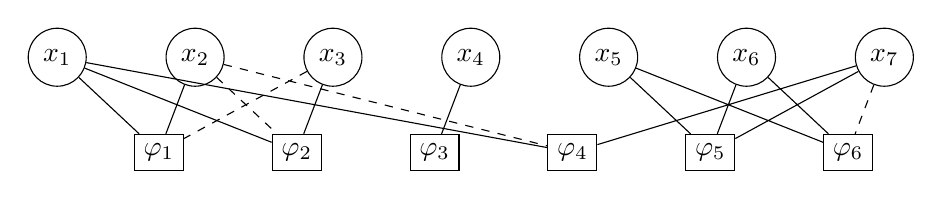
\begin{tikzpicture}
    % Default actions for each node
    \tikzstyle{every node}=[draw, shape=circle];
    % Define and draw five nodes
    \node (v1) {$x_1$};
    \node (v2) [right=1cm of v1] {$x_2$};
    \node (v3) [right=1cm of v2] {$x_3$};
    \node (v4) [right=1cm of v3] {$x_4$};
    \node (v5) [right=1cm of v4] {$x_5$};
    \node (v6) [right=1cm of v5] {$x_6$};
    \node (v7) [right=1cm of v6] {$x_7$};
    \node [rectangle] (c1) [below right=1cm of v1]{$\varphi_1$};
    \node [rectangle] (c2) [below right=1cm of v2]  {$\varphi_2$};
    \node [rectangle] (c3) [below right=1cm of v3]  {$\varphi_3$};
    \node [rectangle] (c4) [below right=1cm of v4]  {$\varphi_4$};
    \node [rectangle] (c5) [below right=1cm of v5]  {$\varphi_5$};
    \node [rectangle] (c6) [below right=1cm of v6]  {$\varphi_6$};

    % Draw radial edges
    \draw [dashed] (v2) -- (c4) (v3) -- (c1) (v2) -- (c2)
    (v7) -- (c6);
    \draw  (v1) -- (c1) (v1) -- (c2) (v1) -- (c4)
            (v2) -- (c1) (v3) -- (c2) (v4) -- (c3)
            (v5) -- (c6) (v6) -- (c5) (v6) -- (c6)
            (v5) -- (c5) (v7) -- (c4) (v7) -- (c5);
    \end{tikzpicture}
\end{figure}

In fact, there are conflicts if every Whiten Variables is changed.
Our approach will eliminate conflicts. $RL$ is $\{\langle x_3, \{\varphi_2\}\rangle, \langle x_5, \{\varphi_5, \varphi_6\} \rangle, \langle x_6, \{\varphi_5, \varphi_6\}\rangle, \langle x_7, \{\varphi_4, \varphi_5\}\rangle, \langle x_1, \{\varphi_1, \varphi_2, \varphi_4\}\rangle\}$, $CAN$ is \{1, 2, 0, 2, 3, 2\}.
Whiten Variables is selected in the order of $x_2$, $x_3$, $x_5$. $x_1$ is added to Frozen Variables because $CAN[1]=1$. After changing $x_2$, $x_3$ and $x_5$, $CAN$ is \{1, 1, 0, 1, 1, 1\}, $x_6$ can't be changed any more.


\section{Experiments results}\label{sec:expr}

The experimental study compared the presented \tool algorithm with respect to the state of the art cb100.

The benchmark consists two parts: the first one are formulae from industrial verification and the second one are random formulae. The industrial formulae are selected from SAT competition between 2002 and 2015. There are 769 industrial formulae out of 1318 formulae in these benchmarks. 388 formulae are selected from industrial formulae that a model can returned from MINISAT in 1800 seconds. The random formulae are generated from unsatisfiable random formulae using the tool of LBX \cite{MPA2015} with over 6000 formulae. For every random formulae, both \tool and cb100 are able to terminate within 1800 seconds.

In Table \ref{tab:ind}, we present the results of industrial formulae. Figure \ref{fig:ind-time} presents a plot by increasing running time of industrial instances for \tool and cb100. We categories the random benchmark into 5 groups, according to the community structure of the formula. Table 3 shows the total SAT solving time, average SAT solving time and average SAT solver call for all 3 groups. In each group, we randomly sample 20 instances and presents a plot by increasing run times in Figure \ref{fig:mcs-time}.

All algorithms introduced in this paper have been implemented in \tool, written in C++ interfacing Minisat 2.2 \cite{MINISAT}.

The experiments were conducted on a cluster of IBM iDataPlex 2.83 GHz, each instance was running with a timeout of 1800 seconds and memory limit of 8 GB.


\subsection{Industrial Experimental Results}

\begin{table*}
\centering
\begin{tabular}{ccccc}
\toprule
 &SAT Solving time&\#SAT Solving Count&Average SAT Solving Time\\
\midrule
\tool&26663 seconds &272089&0.9890 seconds\\
cb100&30295 seconds&239112&1.0174 seconds\\
\bottomrule
\end{tabular}
\caption{Experimental Results for 138 Industrial Formulae}
\label{tab:ind}
\end{table*}

SAT competitions evaluate the performance of SAT solvers, they focused on industrial formula, also contain random formulae or crafted large formulae. We select 769 industrial formulae from all benchmarks, and select 388 formulae that MINISAT return a model in 1800 seconds. The formulae are from different applications of practical, including planning, coloring, hardware/software verification, model checking and cryptanalysis.

Table \ref{tab:ind} shows the overview of industrial benchmark results. Among all the 388 instances, there are 138 instances that both \tool and cb100 were able to compute backbone within 1800 seconds.

Figure 1 provide the performance of \tool and cb100 for industrial formulae, including the time that SAT solver need to generate the first model and total SAT solving time. The first observation is that for instances that need a longer time to generate the first model, \tool outperforms cb100 in both total SAT solving time and average SAT solving time. This implies that \tool is more feasible for large formulae and reduce the complexity of SAT solving for hard formulae. For example, \tool is twice faster than cb100 when computing a formula form \emph{manthey} class. Only for formula in \emph{srhd}, \tool needed 28 more seconds than cb100 does to compute backbone, with a first SAT solving time of 437 seconds.

Another conclusion is that for formulae with first SAT solving time less than 30 seconds, \tool and cb100 are compatible, with only a few seconds more than cb100 does. cb100 highly rely on the quality of model returned by SAT solver, it performances better when SAT solver gave it a suitable model. For most of the formulae that need less than 1 second to compute a first model, both \tool and cb100 were able to compute backbone very quickly with barely difference.

In general \tool performances better than cb100 on industrial instances, especially for instances with a longer time to generate the first model, \tool have a notable advantage. Figure \ref{fig:ind-time} depicts the total SAT solving time of \tool and cb100 by increasing running time of cb100 for the 138 formulae. The line represents the time that a formula need to generate the first model, the running time of \tool are lines with crosses and the running time of cb100 are lines with boxes. It's easy to see that for all formulae that need 120 more seconds to generate the first model, \tool outperforms cb100.

\begin{figure}
    \centering
    \includegraphics[scale=0.7]{ind2.pdf}
   \caption{Total time use for formulae from industrial}
   \label{fig:ind-time}
\end{figure}

\subsection{MSS Extraction Experimental Results}
In this section, the effectiveness of \tool and cb100 for MSS instances are presented.
Unlike other study that focus on the verification instances from industrial, we also study the performance of \tool and cb100 on random instances.
We propose a novel method to generate large number of random formulae, with the help of Maximal Satisfiable Subset(MSS).

Given an unsatisfiable formula $\Phi$, a subset of clauses $\Phi'\subset\Phi$ is called a MSS iff for every clause $\phi\notin\Phi'$, $\Phi'$ is satisfiable and $\Phi'\wedge\phi$ is unsatisfiable. MSS is maximal satisfiable sub-formula extracted from an unsatisfiable formula. There exist a large number of different MSS for a given unsatisfiable formula. We use LBX tool to generate MSSes from random unsatisfiable benchmark. The MSS generated are also random and with a fixed upper bound of clauses count and variables count to a given unsatisfiable formula.

Table \ref{tab:mcs} presents the overview result of MSS formulae. Inspired by the result of industrial formulae, we category MSS formulae into 5 groups according to the computing time of first model. We randomly choose 20 instances from every group and present the running time plot in Figure \ref{fig:mcs-bad}. It's strange that for random formulae, there is no clear relation between the performance of backbone computing and the computing time of first model. It's because that random formulae have more complex community structures \cite{}. We use SATGraph \cite{} tool to generate a graph of a formula. We call a formula with a complex structure if the clusters in the graph are interwind.

\begin{figure}
    \centering
    \includegraphics[scale=0.7]{mcs.pdf}
   \caption{Total time use for formulae from MCS computing}
   \label{fig:mcs-time}
\end{figure}



The results reveal that \tool is as efficiency as cb100 in general. For dense backbones formulae, \tool needs less total SAT solver time. The experiment results present that \tool outperforms cb100 with MSS formulae that generated from unsatisfiable formulae. It's because that \tool is more efficient when dealing with dense backbones. As a result, for dense backbones, \tool is better, no matter the formula is from MSS computing, practical verification or crafted.
As discussed above, for unsatisfiable formulae, the density of backbones will increase simultaneously with the size of MSS formula. In the application of hardware model checking, planning and fault localization, the backbones are dense. With a proper use of other techniques, \tool will reach better performance in application.





\section{Conclusion}\label{sec:conc}
This paper propose a novel greedy-whitening based approach \tool to compute backbone of a propositional formulae. 
\tool comprise with two parts, a greedy based part to compute the under-approximation of backbone of a formula, and an whitening-based part to compute the approximation of backbone. The exact backbone is computed by applying iteratively checking on the approximations. We implements \tool and evaluate it on both industrial formulae with a number of 138 and random formulae with a number of 6606 compared to state of art cb100. Experiment results demonstrate that \tool is able to reduce 11\% running time comparing to cb100. Moreover, for hard random formulae, \tool is able to cut off 40\% running time.



\newpage


\bibliographystyle{plain}
\bibliography{bib}

\end{document}
